\documentclass[12pt,twoside,fleqn,a4paper]{article}
\usepackage[T1]{fontenc}
\usepackage[utf8]{inputenc}

 \usepackage[english]{babel} 
 
\usepackage[a4paper,hdivide={30mm,*,30mm},vdivide={30mm,*,30mm}]{geometry}
\usepackage{amsmath,amssymb,amsfonts,amsthm}
\usepackage{graphics}
\usepackage{graphicx}
\usepackage{eurosym} 
\usepackage{fancyhdr}
\usepackage{color}
\usepackage{setspace}
\usepackage{lmodern} 
\usepackage{textcomp,gensymb} 
\usepackage{subfig} 
\usepackage{calc}
\usepackage{rotating}
\usepackage{placeins}
\usepackage{changepage}
\usepackage{units}

% Comments/modifications
\usepackage{color}
\newcommand{\lp}[1]{{\color{red} #1}}  % Lars Pastewka

% Formatting settings
\singlespacing


%%%%%%%%%%%%%%%%%%%%%%%%%%%%%%%%%%%%%%%%%%%%%%
\begin{document}

\thispagestyle{empty}
\parindent=0mm

\vspace*{10mm}
{\Large Curriculum proposal}
\vspace*{15mm}

{\Large\bf  BSc in Engineering Science}

\vspace*{15mm}
Hans Zappe

\vspace*{15mm}

v. 1 -- \today
\vfill
{\small\parskip-1ex \setcounter{tocdepth}{1}\tableofcontents}~


%%%%%%%%%%%%%%%%%%%%%%%%%%%%%%%%%%%%%%%%%%%%%%
\newpage
\setlength{\parindent}{1em}
\setlength{\parskip}{0em}
\setcounter{page}{1}

\begin{figure}[h]
\centering
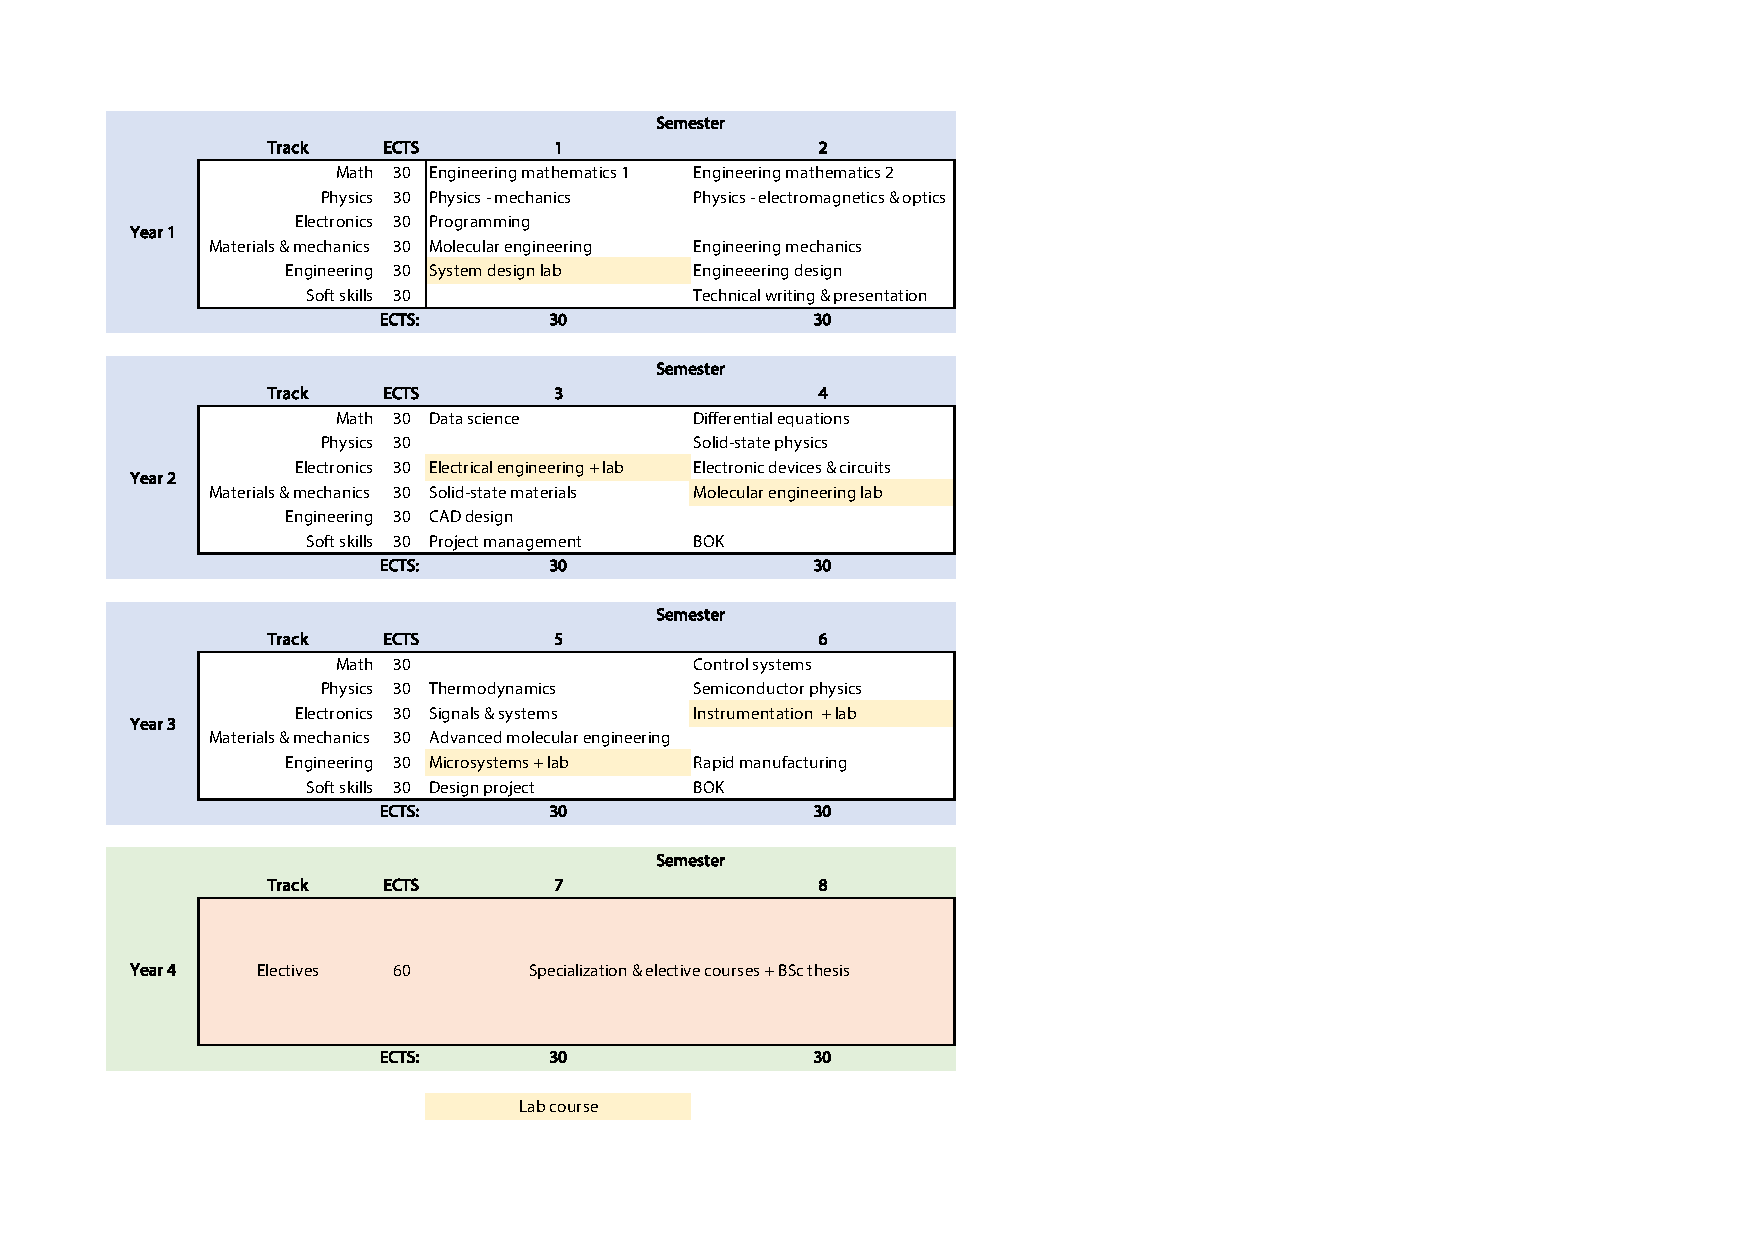
\includegraphics[width=0.9\columnwidth]{CoreCurriculumGraphic}
\caption{Summary of the BSc Engineering Science core curriculum \& electives}
\label{pic:Single}
\end{figure}



%%%%%%%%%%%%%%%%%%%%%%%%%%%%%%%%%%%%%%%%%%%%%%
\newpage
\section{Math track}
\begin{description}
\item[Responsible:] Pastewka
\end{description}
\vspace{1 mm}


%%%%%%%%%%%%%%%%%%%%%
\subsection{Engineering mathematics 1}
\begin{tabular}{llll} \hline
\textbf{Semester:} 1 & \textbf{ECTS:} 6 & \textbf{Lab:} no & \textbf{Possible instructors:} ?\\
\hline
\end{tabular}

\begin{itemize}
\setlength\itemsep{0cm}
\item Fundamentals of logic
\begin{itemize}
    \item Sets
    \item Propositions and propositional calculus 
    \item Algebraic structures
    \item Boolean algebra
\end{itemize}
\item Numbers
\begin{itemize}
    \item Natural numbers and integers
    \item Rational numbers
    \item Real and complex numbers
\end{itemize}

\item Linear Algebra
\begin{itemize}
    \item Vector spaces
    \item Linear independence, bases, dimension
    \item Scalar product and metric
    \item Systems of linear equations
    \item Gaussian elimination
    \item Relation of the solution of linear systems to vector spaces
    \item Determminants and matrices
    \item Rank of matrices, quadratic matrices
    \item Spectrum and normal forms of quadratic matrices
    \item Tensors and matrices
\end{itemize}
\end{itemize}


%%%%%%%%%%%%%%%%%%%%%
\subsection{Engineering mathematics 2}
\begin{tabular}{llll} \hline
\textbf{Semester:} 2 & \textbf{ECTS:} 6 & \textbf{Lab:} no & \textbf{Possible instructors:} ?\\
\hline
\end{tabular}

\begin{itemize}
\setlength\itemsep{0cm}
\item Calculus
\begin{itemize}
    \item Functions of one and multiple variables
    \item Differentiation, one and multiple variables
    \item Integration, one and multiple variables
    \item Convergence, limits and series
    \item Normed vector spaces
    \item Integral transforms: Fourier and Laplace
\end{itemize}
\item Tensoranalysis
\begin{itemize}
    \item Differentiation of vector fields
    \item Divergence, curl, and gradient
    \item Field lines, Gauß' and Stokes' theorem
\end{itemize}
\end{itemize}


%%%%%%%%%%%%%%%%%%%%%
\subsection{Data science}
\begin{tabular}{llll} \hline
\textbf{Semester:} 3 & \textbf{ECTS:} 6 & \textbf{Lab:} no & \textbf{Possible instructors:} Moritz Diehl, Lars Pastewka, Oliver Paul \\
\hline
\end{tabular}

\begin{itemize}
\setlength\itemsep{0cm}
\item \lp{It would be good if data science came after differential equations}
\item Frequentist probability
\item Bayesian probability
\item Stochastic processes (Langevin and Fokker-Planck equations)
\item Parametric Bayesian inference
\item Gaussian processes and nonparametric Bayesian inference
\item Neuronal networks
\end{itemize}


%%%%%%%%%%%%%%%%%%%%%
\subsection{Differential equations}
\begin{tabular}{llll} \hline
\textbf{Semester:} 4 & \textbf{ECTS:} 6 & \textbf{Lab:} yes & \textbf{Possible instructors:} Moritz Diehl, Andreas Greiner, Lars Pastewka \\
\hline
\end{tabular}
\lp{I strongly suggest to put DEs right after engineering math 2}
\begin{itemize}
\setlength\itemsep{0cm}
\item Ordinary Differential Equations
\item Systems of ordinary differential equations
\item Partial Differential Equation
\item Nonlinear Differential Equations
\item Numerical methos
\item Calculus of variations: Variational formulation of dynamical problems
\item Stability of dynamical systems
\item Analysis and visualization of results (Python Lab, goes into all subjects)
\end{itemize}
\lp{Since there will be no more Simulation course I propose to do a lot of hands on DE solving
and visualization with Python$\rightarrow$ needs Programming in 1st term, Python only and to be used throughout the programme.}

%%%%%%%%%%%%%%%%%%%%%
\subsection{Control systems}
\begin{tabular}{llll} \hline
\textbf{Semester:} 6 & \textbf{ECTS:} 6 & \textbf{Lab:} no & \textbf{Possible instructors:} Diehl\\
\hline
\end{tabular}

\begin{itemize}
\setlength\itemsep{0cm}
\item State-Space Modeling of Dynamical Systems
\item Input-Output System Models
\item Stability and Characteristic Polynomial
\item Linear Time Invariant Systems (Step-Response, BIBO Stability, Transfer Function, Bode- and Nyquist-Plot)
\item Feedback Control Architectures
\item Stability of Controlled Systems
\item PID Control
\item Frequency Domain Control Design
\item State Space Control Design (Controllability, Pole Placement, LQR)
\item State Estimation (Observability, Luenberger Observer, Kalman Filter)
\end{itemize}


%%%%%%%%%%%%%%%%%%%%%%%%%%%%%%%%%%%%%%%%%%%%%%
\newpage
\section{Physics track}
\begin{description}
\item[Responsible:] Paul
\end{description}
\vspace{1 mm}


%%%%%%%%%%%%%%%%%%%%%
\subsection{Physics -- mechanics}
\begin{tabular}{llll} \hline
\textbf{Semester:} 1 & \textbf{ECTS:} 6 & \textbf{Lab:} no & \textbf{Possible instructors:} ?\\
\hline
\end{tabular}

\begin{itemize}
\setlength\itemsep{0cm}
\item Massepunkt
\begin{itemize}
\item Orts-, Geschwindigkeits-, Beschleunigungsvektoren
\item Arbeit, Energie, Impuls, Leistung, Erhaltungssätze
\item Reibung
\item Gravitation, Coulomb
\item Trägheitskräfte (Zentrifugalk., Coriolis-K.)
\end{itemize}

\item Starrer Körper
\begin{itemize}
\item Translation, Rotation
\item Trägheitsmoment, Drehmoment, Drehimpuls
\item Drehimpulserhaltung
\item Statische und dynamisches Gleichgewicht
\item Bewegungsgleichungen 
\item Kreisel
\end{itemize}

\item Schwingungen und Wellen
\begin{itemize}
\item Grundgleichung
\item Überlagerung, 1D, mehr-D
\item freie Schwingung, gedämpfte Schwingung
\item erzwungene Schwingung
\item Wellengleichung
\item Elastische Wellen, Seilwellen, Wasserwellen
\item Überlagerung von Wellen
\item Energie von Wellen
\item Streuung, Beugung, Absorption, nichtlineare Phänomenen (Schockwellen)
\item Einfaches Pendel
\item Gekoppelte Pendel
\item Schwingungen von Balken und Platten
\end{itemize}
\end{itemize}


%%%%%%%%%%%%%%%%%%%%%
\subsection{Physics -- electromagnetics \& optics}
\begin{tabular}{llll} \hline
\textbf{Semester:} 2 & \textbf{ECTS:} 6 & \textbf{Lab:} no & \textbf{Possible instructors:} ?\\
\hline
\end{tabular}

\begin{itemize}
\setlength\itemsep{0cm}
\item Elektrizität
\begin{itemize}
\item Elektrostatik
\item Dielektrika: Verschiebungsdichte, Polarisation, Energiedichte
\end{itemize}

\item Elektrodynamik
\begin{itemize}
\item Magnetfeld
\item Kräfte auf Ladungsträger und Ströme im Magnetfeld
\item Erzeugung von Magnetfeldern
\item Induktion
\item Wechselströme
\item Maxwell-Gleichungen
\item Ebene elmag. Wellen
\item Dipolstrahlung
\item Wellenleiter
\end{itemize}

\item Geometrische Optik
\begin{itemize}
\item Reflexion, Brechung, Snellius-Gesetz, totalreflexion
\item Optische Elemente
\item Elektronenoptik
\end{itemize}

\item Wellenoptik
\begin{itemize}
\item Kohärenz
\item Interferenz
\item Beugung am Gitter
\item Spalt- und Lochblende
\item Auflösungsvermögen: Rayleigh
\item Fresnellinsen
\item Fabry-Perot, DBR
\item Lichtpolarisation
\item Absorption von Licht
\item Dispersion von Lichtpulsen
\end{itemize}

\item Strahlungsenergie
\begin{itemize}
\item Strahlungsspektrum
\item Wärmestrahlung
\item Schwarzkörperstrahlung, Stefan-Boltzmann
\item Von IR bis UV
\end{itemize}
\end{itemize}


%%%%%%%%%%%%%%%%%%%%%
\subsection{Solid-state physics}
\begin{tabular}{llll} \hline
\textbf{Semester:} 4 & \textbf{ECTS:} 6 & \textbf{Lab:} no & \textbf{Possible instructors:} ?\\
\hline
\end{tabular}

\begin{itemize}
\setlength\itemsep{0cm}
\item Aubau der Festkörper
\begin{itemize}
\item Übersicht über Atomaufbau und Orbitale
\item Gitteraufbau, Gittervektoren, Basisvektoren
\item Kristallebenen, Miller-Indizes
\item Bravais-Gitter
\item Wichtigste Kristallstrukturen (sc, bcc, fcc, hcp)
\end{itemize}

\item Strukturaufklärung
\begin{itemize}
\item Bragg-Streuung
\item Reziprokes Gitter
\item Laue-Bedingung, Ewald-Konstruktion
\item Röntgen-, Neutronen- Elektronen-Streuung
\item Laue-Methode, Debye-Scherrer-Methode
\end{itemize}

\item Bindung der Festkörper
\begin{itemize}
\item Lennard-Jones-Potenzial
\item van der Waals, Dispersions-Kräfte
\item Ionische Bidung, Madelung
\item Metallische Bindung
\item Kovalente Bindung
\end{itemize}

\item Schwingungszustände des Festkörpers
\begin{itemize}
\item Masse-Feder-Modell
\item Longitudinale und transverse Schwingungen
\item Schwingungsquanten, Phononen
\item Bose-Einstein-Verteilung
\item Schwingungsenergie des Festkörpers und spezifische Wärme
\item Einsteil-Modell der spezifischen Wärme
\item Debye-Modell der spezifischen Wärme
\item Wärmeleitung durch Gitterschwingungen
\end{itemize}

\item Elektronen im Festkörper
\begin{itemize}
\item Schrödingergleichung und Blochzustände
\item Bandstruktur
\item Quasifreie Elektronen
\item Elektronen im periodischen Potenzial: Bänder und Bandlücken
\item Fermiverteilung, Fermifläche
\item Spezifische Wärme der Elektronen
\item Elektrische Leitung im Metall
\item Wiedemann-Franz-Gesetz
\item Halbleiter: Valenz-/Leitungsband, dirrekte/indirekte Bandlücke Elektronen/Löcher, intrinsischer HL, Dotierung)
\item Lichtabsorption im HL
\end{itemize}

\item Magnetismus
\begin{itemize}
\item Magnetisches Moment, Magnetisierung
\item Dia-/Para-/Ferrognetismus
\item Langevinscher Diamagnetismus
\item Langevinscher Paramagnetismus
\item Bandmagnetismus nach Pauli
\item Ferromagnetismus
\end{itemize}
\end{itemize}


%%%%%%%%%%%%%%%%%%%%%
\subsection{Thermodynamics}
\begin{tabular}{llll} \hline
\textbf{Semester:} 5 & \textbf{ECTS:} 6 & \textbf{Lab:} no & \textbf{Possible instructors:} ?\\
\hline
\end{tabular}

\begin{itemize}
\setlength\itemsep{0cm}
\item Wärmeenergie, Temperatur, spezifische Wärme
\item Kinetische Gastheorie
\item Wärmekraftmaschinen
\item Wärmeleitung, Diffusion
\item Entropie, Enthalpie, freie Energie
\item Aggregatszustände, Gibbssche Phasenregel
\end{itemize}


%%%%%%%%%%%%%%%%%%%%%
\subsection{Semiconductor physics}
\begin{tabular}{llll} \hline
\textbf{Semester:} 6 & \textbf{ECTS:} 6 & \textbf{Lab:} no & \textbf{Possible instructors:} ?\\
\hline
\end{tabular}

\begin{itemize}
\setlength\itemsep{0cm}
\item This and that and
\item Semiconductor band structures
\item Electronic transport and transport properties
\item Elementrary excitations in SCs

\end{itemize}


%%%%%%%%%%%%%%%%%%%%%%%%%%%%%%%%%%%%%%%%%%%%%%
\newpage
\section{Electronics track}
\begin{description}
\item[Responsible:] Zappe, Diehl
\end{description}
\vspace{1 mm}


%%%%%%%%%%%%%%%%%%%%%
\subsection{Programming}
\begin{tabular}{llll} \hline
\textbf{Semester:} 1 & \textbf{ECTS:} 6 & \textbf{Lab:} no & \textbf{Possible instructors:} ?\\
\hline
\end{tabular}

\begin{itemize}
\setlength\itemsep{0cm}
\item This and that
\end{itemize}


%%%%%%%%%%%%%%%%%%%%%
\subsection{Electrical engineering}
\begin{tabular}{llll} \hline
\textbf{Semester:} 3 & \textbf{ECTS:} 6 & \textbf{Lab:} yes & \textbf{Possible instructors:} Stieglitz/Kuhl\\
\hline
\end{tabular}

\begin{itemize}
\setlength\itemsep{0cm}
\item Basic circuit elements (R,C,L, diodes)
\item Sources
\item dc network analysis
\item Fourier analysis
\item ac network analysis, frequency response, \& switching
\item Feedback networks
\item Digital systems
\item Electrical power, electromagnetism \& transformers
\item Electromechanics
\end{itemize}


%%%%%%%%%%%%%%%%%%%%%
\subsection{Electronic devices \& circuits}
\begin{tabular}{llll} \hline
\textbf{Semester:} 4 & \textbf{ECTS:} 6 & \textbf{Lab:} yes & \textbf{Possible instructors:} Zappe\\
\hline
\end{tabular}

\begin{itemize}
\setlength\itemsep{0cm}
\item Bipolar transistors \& MOSFETs
\item Bipolar circuit analysis
\item Bipolar single-stage, differential, multi-stage \& power amplifiers
\item Filters, signal generators \& current sources
\item Op amps
\item MOSFET circuit analysis
\item MOS digital logic circuits
\item Digital memory
\item Microelectronics \& integrated circuits
\item Circuit simulation
\end{itemize}


%%%%%%%%%%%%%%%%%%%%%
\subsection{Signals \& systems}
\begin{tabular}{llll} \hline
\textbf{Semester:} 5 & \textbf{ECTS:} 6 & \textbf{Lab:} no & \textbf{Possible instructors:} Diehl\\
\hline
\end{tabular}

\begin{itemize}
\setlength\itemsep{0cm}
\item Signals \& spectral analysis
\item Impulse \& frequency response, transfer functions
\item Fourier analysis \& FFT
\item Time and transform-domain representations
\item Sampling, convolution, deconvolution, quantizing
\item Noise, filtering \& compression
\item Probabilistic models; stochastic processes
\item Correlation functions, power spectra, spectral factorization
\end{itemize}


%%%%%%%%%%%%%%%%%%%%%
\subsection{Instrumentation}
\begin{tabular}{llll} \hline
\textbf{Semester:} 6 & \textbf{ECTS:} 6 & \textbf{Lab:} yes & \textbf{Possible instructors:} Rupitsch\\
\hline
\end{tabular}

\begin{itemize}
\setlength\itemsep{0cm}
\item Sensors \& signal types
\item Sampling \& measurement error
\item Fourier transforms, impulse response, transfer functions, linear time-invariant systems
\item Measurement concepts, filters, A/D \& D/A conversion
\item Analog \& digital measurement systems
\item Example measurement systems
\begin{itemize}
\item Position, velocity \& rotation measurement
\item Temperature, force \& pressure measurement
\end{itemize}
\end{itemize}


%%%%%%%%%%%%%%%%%%%%%%%%%%%%%%%%%%%%%%%%%%%%%%
\newpage
\section{Materials \& mechanics track}
\begin{description}
\item[Responsible:] Rühe, Rapp
\end{description}
\vspace{1 mm}


%%%%%%%%%%%%%%%%%%%%%
\subsection{Molecular engineering}
\begin{tabular}{llll} \hline
\textbf{Semester:} 1 & \textbf{ECTS:} 6 & \textbf{Lab:} no & \textbf{Possible instructors:} Rapp/Rühe\\
\hline
\end{tabular}

\begin{itemize}
\setlength\itemsep{0cm}
\item Atommodelle
\item Chemische Bindung
\item Phasen
\item Stöchiometrie
\item pH-Werte
\item Massentransport
\item Elektrochemie
\item Analytische Verfahren (IR,NMR...)
\end{itemize}


%%%%%%%%%%%%%%%%%%%%%
\subsection{Engineering mechanics}
\begin{tabular}{llll} \hline
\textbf{Semester:} 2 & \textbf{ECTS:} 6 & \textbf{Lab:} no & \textbf{Possible instructors:} Woias\\
\hline
\end{tabular}

\begin{itemize}
\setlength\itemsep{0cm}
\item This and that
\end{itemize}


%%%%%%%%%%%%%%%%%%%%%
\subsection{Solid-state materials}
\begin{tabular}{llll} \hline
\textbf{Semester:} 3 & \textbf{ECTS:} 6 & \textbf{Lab:} no & \textbf{Possible instructors:} Paul\\
\hline
\end{tabular}

\begin{itemize}
\setlength\itemsep{0cm}
\item This and that
\end{itemize}


%%%%%%%%%%%%%%%%%%%%%
\subsection{Molecular engineering lab}
\begin{tabular}{llll} \hline
\textbf{Semester:} 4 & \textbf{ECTS:} 6 & \textbf{Lab:} yes & \textbf{Possible instructors:} Rühe\\
\hline
\end{tabular}

\begin{itemize}
\setlength\itemsep{0cm}
\item Analysis
\item Synthesis
\item Project-oriented connection to engineering problem
\end{itemize}


%%%%%%%%%%%%%%%%%%%%%
\subsection{Advanced molecular engineering}
\begin{tabular}{llll} \hline
\textbf{Semester:} 5 & \textbf{ECTS:} 6 & \textbf{Lab:} no & \textbf{Possible instructors:} multiple\\
\hline
\end{tabular}

\begin{itemize}
\setlength\itemsep{0cm}
\item Polymere / Soft Matter
\begin{itemize}
\item concepts in soft matter / polymers
\item smart, responsive materials
\item bioinspired materials
\item light weight composites
\end{itemize}

\item Molecular Bioengineering
\begin{itemize}
\item Biosensors
\item Biomaterials
\item Bioengineering: From biointerfaces to Regenerative Medicine
\end{itemize}

\item Molecular Engineering for sustainable solutions
\begin{itemize}
\item Energy conversion and storage
\item Water purification
\item From Cradle to cradle: Materials Cycles
\item biobased Materials; Biodegradation
\end{itemize}

\item Computational
\begin{itemize}
\item skalenübergreifende Modellierung
\end{itemize}
\end{itemize}


%%%%%%%%%%%%%%%%%%%%%%%%%%%%%%%%%%%%%%%%%%%%%%
\newpage
\section{Engineering track}
\begin{description}
\item[Responsible:] Woias
\end{description}
\vspace{1 mm}


%%%%%%%%%%%%%%%%%%%%%
\subsection{System design lab}
\begin{tabular}{llll} \hline
\textbf{Semester:} 1 & \textbf{ECTS:} 6 & \textbf{Lab:} yes & \textbf{Possible instructors:} Rupitsch\\
\hline
\end{tabular}

\begin{itemize}
\setlength\itemsep{0cm}
\item This and that
\end{itemize}


%%%%%%%%%%%%%%%%%%%%%
\subsection{Engineering design}
\begin{tabular}{llll} \hline
\textbf{Semester:} 2 & \textbf{ECTS:} 6 & \textbf{Lab:} no & \textbf{Possible instructors:} Woias\\
\hline
\end{tabular}

\begin{itemize}
\setlength\itemsep{0cm}
\item This and that
\end{itemize}


%%%%%%%%%%%%%%%%%%%%%
\subsection{CAD design}
\begin{tabular}{llll} \hline
\textbf{Semester:} 3 & \textbf{ECTS:} 6 & \textbf{Lab:} no & \textbf{Possible instructors:} ?\\
\hline
\end{tabular}

\begin{itemize}
\setlength\itemsep{0cm}
\item This and that
\end{itemize}


%%%%%%%%%%%%%%%%%%%%%
\subsection{Microsystems}
\begin{tabular}{llll} \hline
\textbf{Semester:} 5 & \textbf{ECTS:} 6 & \textbf{Lab:} yes & \textbf{Possible instructors:} Wallrabe/Zengerle\\
\hline
\end{tabular}

\begin{itemize}
\setlength\itemsep{0cm}
\item This and that
\end{itemize}


%%%%%%%%%%%%%%%%%%%%%
\subsection{Rapid manufacturing}
\begin{tabular}{llll} \hline
\textbf{Semester:} 6 & \textbf{ECTS:} 6 & \textbf{Lab:} no & \textbf{Possible instructors:} ?\\
\hline
\end{tabular}

\begin{itemize}
\setlength\itemsep{0cm}
\item Stereolithographie
\item 3D-Druck mittels FDM (Fused Deposition modeling)
\item Lasermikrobearbeitung
\item CAM (Computer-Aided Manufacturing)

\end{itemize}


%%%%%%%%%%%%%%%%%%%%%%%%%%%%%%%%%%%%%%%%%%%%%%
\newpage
\section{Soft skills track}
\begin{description}
\item[Responsible:] ?
\end{description}
\vspace{1 mm}


%%%%%%%%%%%%%%%%%%%%%
\subsection{Technical writing \& presentation}
\begin{tabular}{llll} \hline
\textbf{Semester:} 2 & \textbf{ECTS:} 6 & \textbf{Lab:} no & \textbf{Possible instructors:} Hanemann\\
\hline
\end{tabular}

\begin{itemize}
\setlength\itemsep{0cm}
\item This and that
\end{itemize}


%%%%%%%%%%%%%%%%%%%%%
\subsection{Project management}
\begin{tabular}{llll} \hline
\textbf{Semester:} 3 & \textbf{ECTS:} 6 & \textbf{Lab:} no & \textbf{Possible instructors:} Wallrabe\\
\hline
\end{tabular}

\begin{itemize}
\setlength\itemsep{0cm}
\item This and that
\end{itemize}


%%%%%%%%%%%%%%%%%%%%%
\subsection{BOK}
\begin{tabular}{llll} \hline
\textbf{Semester:} 4 & \textbf{ECTS:} 6 & \textbf{Lab:} no & \textbf{Possible instructors:} external\\
\hline
\end{tabular}

\begin{itemize}
\setlength\itemsep{0cm}
\item This and that
\end{itemize}


%%%%%%%%%%%%%%%%%%%%%
\subsection{Design project}
\begin{tabular}{llll} \hline
\textbf{Semester:} 5 & \textbf{ECTS:} 6 & \textbf{Lab:} yes & \textbf{Possible instructors:} all labs\\
\hline
\end{tabular}

\begin{itemize}
\setlength\itemsep{0cm}
\item This and that
\end{itemize}


%%%%%%%%%%%%%%%%%%%%%
\subsection{BOK}
\begin{tabular}{llll} \hline
\textbf{Semester:} 6 & \textbf{ECTS:} 6 & \textbf{Lab:} no & \textbf{Possible instructors:} external\\
\hline
\end{tabular}

\begin{itemize}
\setlength\itemsep{0cm}
\item This and that
\end{itemize}


\end{document}
